\section{Data Analysis}

\subsection{Matrix Multiplication}
In this section, we will focus on the Matrix Multiplication algorithm. All experiments shown will have been run with a matrix multiplication lambda function in a HPX $for\_each()$ The goal is to start analyzing a smaller data set before slowly expanding it by adding new lambda functions. In the case of a matrix multiplication algorithm the feature <Input-size> can be renamed <Matrix Size>.

\subsubsection{Variance of execution times for a given chunk-size}
For a given experiment, you expect to get similar execution times for a given chunk size value every time you run it. There will always be some noise in the data since there are many processes that the user cannot directly control. To correct that, every for-loop is run $N_\text{rep}$ times and the execution time is given by the mean of these repetitions. Each repetition can be represented by an index $j=0,1,2,3,4, \dots$ So for an experiment $i$ the execution time outputted is 
$$\bar{t}_i=\frac{1}{N_\text{rep}}\sum_{j=1}^{N_\text{rep}}t_j$$
Note that the first repetition of the for-loop is ignored so this repetition could be given an index $j=0$. This is done to ignore the time where the cache memory is being filled.
One would expect the variance of the mean
to decrease as the number of repetitions get bigger. If this could be confirmed experimentally, this would mean that by taking more and more repetitions, one can get more precise in execution time measurement and therefore the data generation process described earlier can be reliable. Studying the variance is a great tool to measure the variations of execution time between repetitions but it does not inform on how much the values vary relative to their size. To solve this issue, the relative variance is used:
$$\operatorname{RelVAR}(\bar{t}_j)=\frac{\operatorname{VAR}(\bar{t}_j)}{\bar{t}_j^2}\times 100 \%$$

To test this assertion, the relative variance of the mean of execution times has been measured for values of $N_{rep}=10,25,50,75,100$. These measurements have been done on matrix multiplications algorithms with different number of threads and different matrix sizes
\begin{figure*}
	\centering
	\begin{subfigure}[b]{0.475\textwidth}
		\centering
		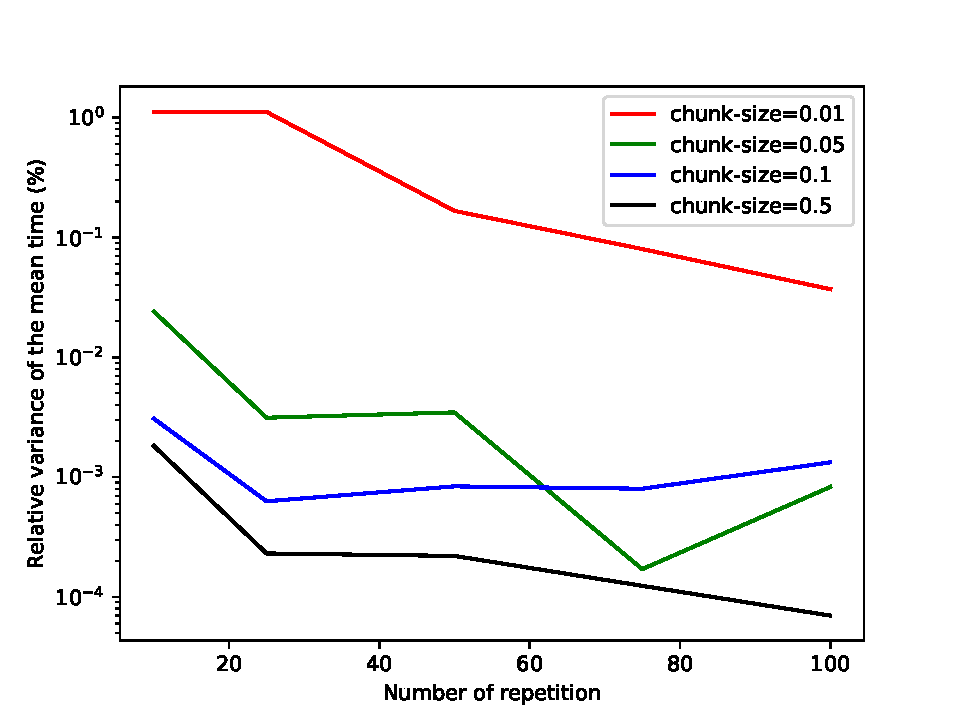
\includegraphics[width=\textwidth]{images/relvar_100_2.pdf}
		\caption[Network2]%
		{{\small 100$\times$100 on 2 threads}}    
	\end{subfigure}
	\hfill
	\begin{subfigure}[b]{0.475\textwidth}  
		\centering 
		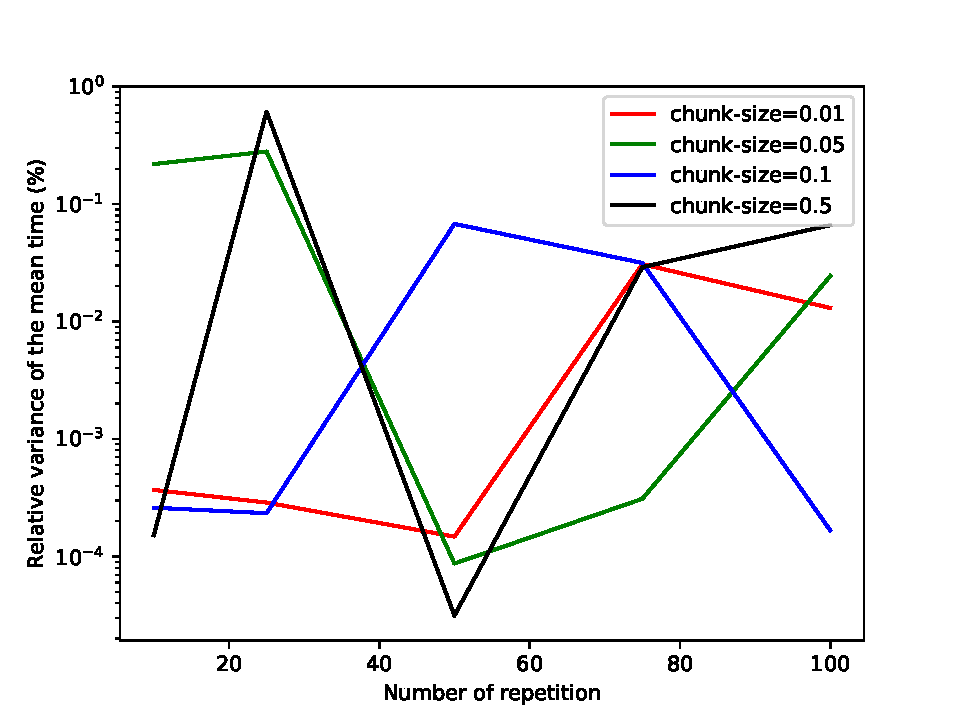
\includegraphics[width=\textwidth]{images/relvar_500_2.pdf}
		\caption[]%
		{{\small 500$\times$500 on 2 threads}}    
	\end{subfigure}
	\vskip\baselineskip
	\begin{subfigure}[b]{0.475\textwidth}   
		\centering 
		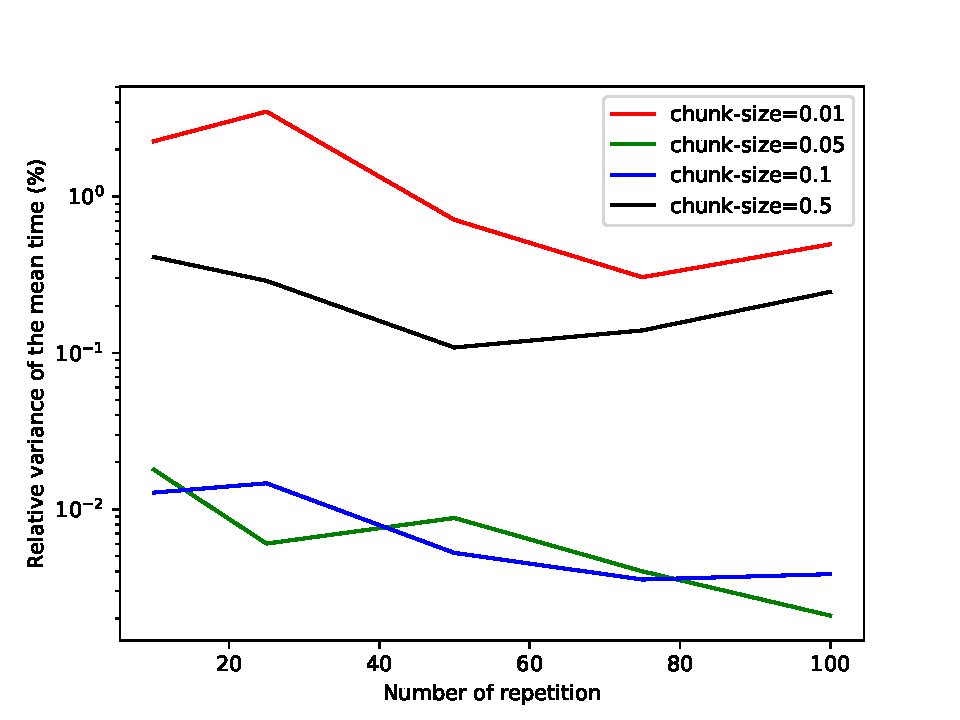
\includegraphics[width=\textwidth]{images/relvar_100_4.pdf}
		\caption[]%
		{{\small 100$\times$100 on 4 threads}}    
	\end{subfigure}
	\quad
	\begin{subfigure}[b]{0.475\textwidth}   
		\centering 
		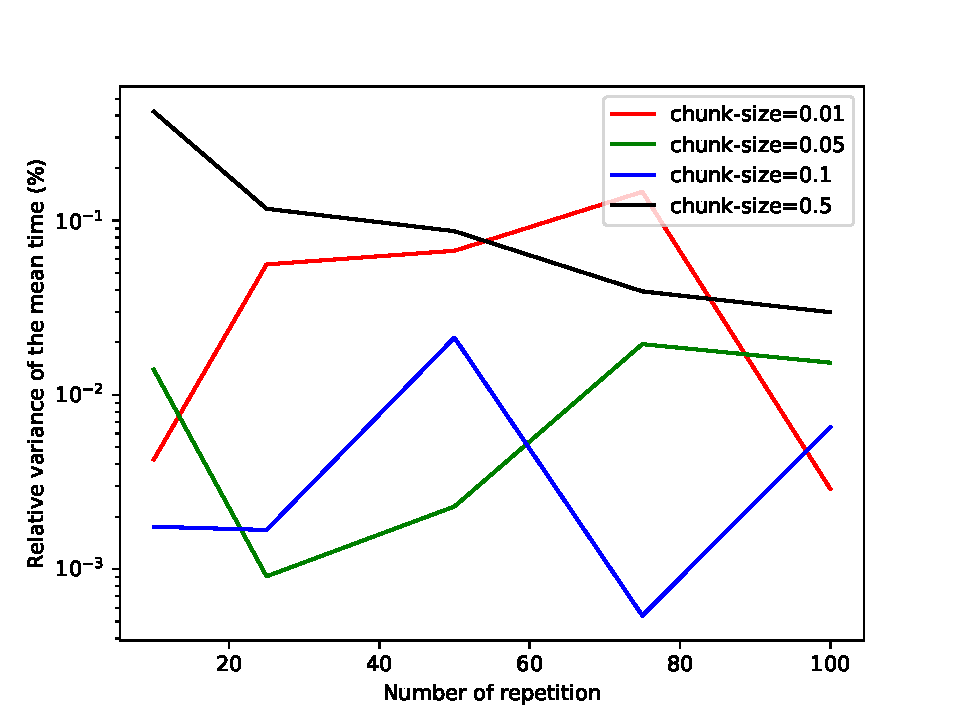
\includegraphics[width=\textwidth]{images/relvar_500_4.pdf}
		\caption[]%
		{{\small 500$\times$500 on 4 threads}}    
	\end{subfigure}
	\vskip\baselineskip
	\begin{subfigure}[b]{0.475\textwidth}   
		\centering 
		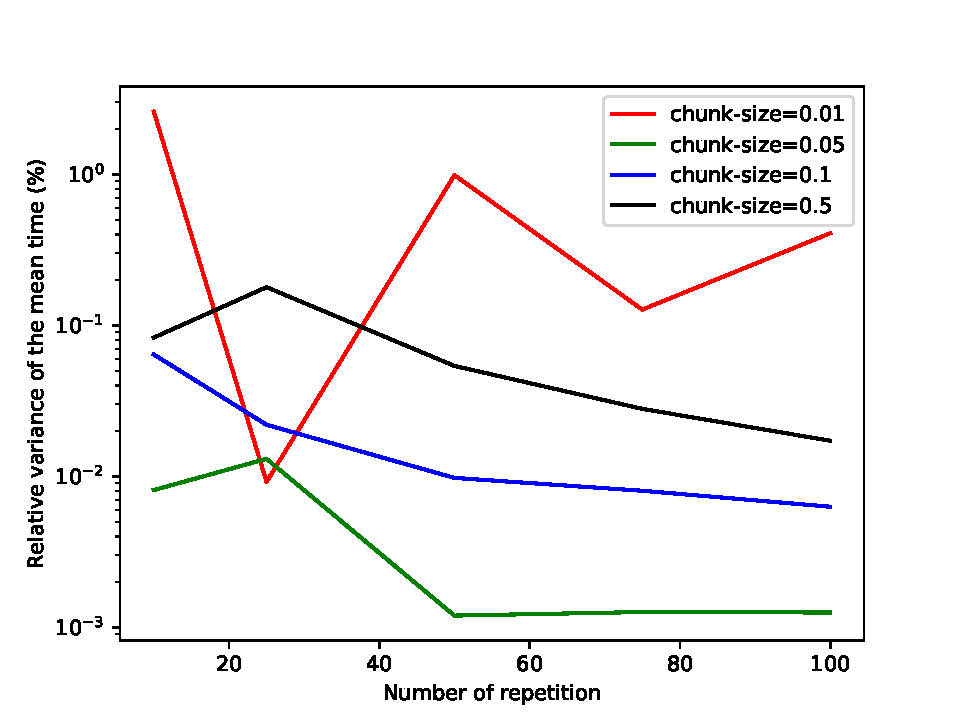
\includegraphics[width=\textwidth]{images/relvar_100_8.pdf}
		\caption[]%
		{{\small 100$\times$100 on 8 threads}}    
	\end{subfigure}
	\quad
	\begin{subfigure}[b]{0.475\textwidth}   
		\centering 
		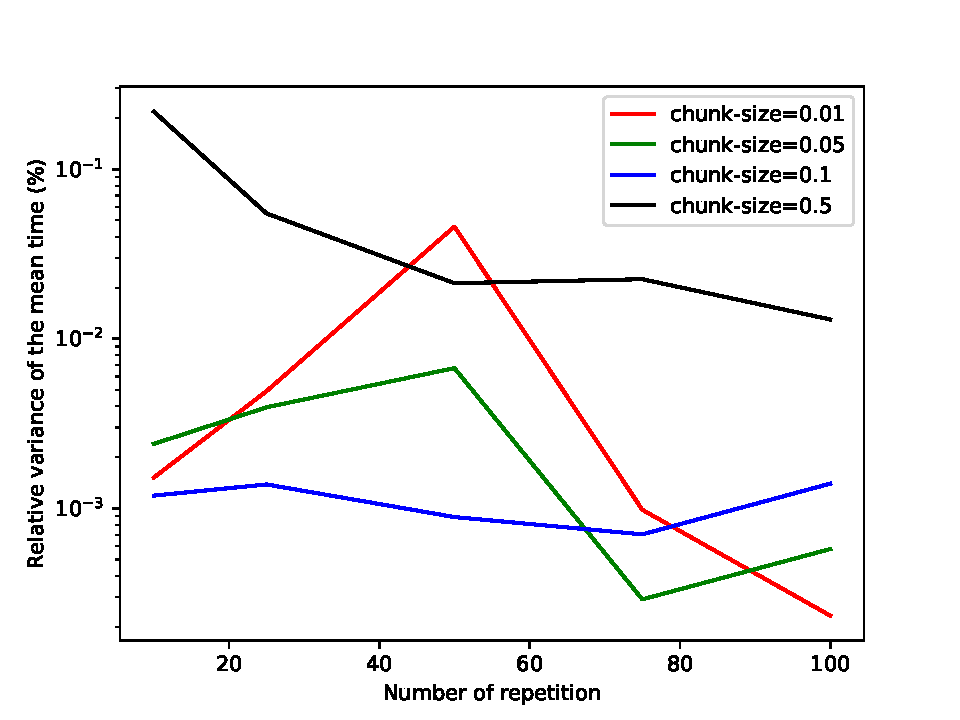
\includegraphics[width=\textwidth]{images/relvar_500_8.pdf}
		\caption[]%
		{{\small 500$\times$500 on 8 threads}}    
\end{subfigure}
	\caption[Standard deviations]
	{\small Variances of the mean of execution times for different experiments  and different chunk sizes on Matrix Multiplication algorithm} 

\end{figure*}
\newpage
From this analysis, we can see that in most cases for a 100x100 matrix the variance of the mean get smaller when $N_{rep}$ get bigger which ultimately means that the more repetitions you do when generating your data, the more accurate your execution time measurement becomes. There are oscillations in some cases, mostly with 500x500 matrices, but the relative variances is always smaller or close to 1\% (the maximal relative variance measure was 2\%). Since the relative variance is always smaller or close to 1\%,even for 10 repetitions, it was decided that 10 repetitions would be enough for this work. This means that every time I run any experiment, I measure the execution time of a HPX for-loop 10 times and output the mean. This choice was made to accelerate the data generation process but a larger number of repetitions can be used to generate more precise data at the cost of time.

\subsubsection{Variations of optimal chunk size for a given experiment}

Now that it has been demonstrated that you can accurately measure execution time by having more and more repetitions, one would expect the optimal chunk size to be the same each time you run the same experiment. This is important because the goal of the project is to predict the optimal chunk-size based on the features of a loop. If you run an experiment twice and get different optimal chunk sizes, than it would mean that there is no function $$f:\{X_i\} \rightarrow cs_i$$ 

 . It is important to be sure that such a function can exist because this is the function that will be approximated with machine learning. To analyze the variations in optimal chunk size, the same experiments as previous section have been run. Chunk sizes of \{0.01,0.05,0.1,0.5\} have once again been used on loops with 100 and 500 iterations with 2,4 and 8 threads. Here are the optimal chunk sizes for each experiment.Each column represents an experiment and each row represents a repetition on the given experiment.
\begin{table}[H]
	\centering
	\caption{Optimal Chunk size for repetitions of matrix multiplication experiments}
	\label{my-label}
	\begin{tabular}{|c|c|c|c|c|c|c|}
		\hline
		&
		\multicolumn{2}{|c|}{2 Threads} & \multicolumn{2}{c|}{4 Threads} & \multicolumn{2}{c|}{8 Threads} \\ \hline
		experiment&100x100       & 500x500       & 100x100       & 500x500      & 100x100       & 500x500      \\ \hline
		1&0.5            & 0.5            & 0.5            & 0.01          & 0.05           & 0.5           \\ \hline
		2&0.5            & 0.5            & 0.1            & 0.05          & 0.05           & 0.05          \\ \hline
		3&0.5            & 0.5            & 0.1            & 0.05          & 0.05           & 0.5           \\ \hline
		4&0.5            & 0.5            & 0.1            & 0.05          & 0.01           & 0.01          \\ \hline
		5&0.5            & 0.5            & 0.1            & 0.05          & 0.05           & 0.01          \\ \hline
		6&0.5            & 0.5            & 0.1            & 0.05          & 0.05           & 0.01          \\ \hline
		7&0.5            & 0.5            & 0.1            & 0.05          & 0.05           & 0.01          \\ \hline
		8&0.5            & 0.5            & 0.5            & 0.05          & 0.05           & 0.01          \\ \hline
		9&0.5            & 0.5            & 0.1            & 0.01          & 0.01           & 0.01          \\ \hline
		10&0.5            & 0.5            & 0.1            & 0.5           & 0.05           & 0.01          \\ \hline
	\end{tabular}
\end{table}

As we can see there are some variations in optimal chunk size when you run the same experiment different times and therefore we are not guaranteed to find the same target values when re-generating data. However, for these tests, we can clearly identify a value for chunk size that is selected more often than the other values. To conclude, the function $f$ does seem to exist but with some background noise.

\subsubsection{Comparison of executions times for all chunk size candidates}
As seen previously, when you run the same experiment multiple times, there is some variation in the optimal chunk size obtained. To understand this in more details, I decided to analyze the variations of execution times with respect to different chunk size candidates.
 In fact, for experiments where there is very little variations in executions times for different chunk-sizes, we should expect huge variations in optimal chunk-size since the times are so close that the optimal chunk size keeps changing.

One way to study the variations between execution times for different chunk sizes is the variance. Here the variance is calculated by the following for an experiment $i$:
$$\operatorname{VAR}(t_i)=\frac{1}{Card(CS)-1}\sum_{cs \in CS}(t(X_i,cs)-\bar{t}_i)^2$$
with 
$$\bar{t}_i=\frac{1}{Card(CS)}\sum_{cs \in CS}t(X_i,cs)$$

 $Card(CS)$ is the cardinality of the set $CS$ which means how many candidates are being tested. Also, in that case the mean $\bar{t}_i$ is the average of executions times between all chunk sizes candidates. This variance can be interpreted as how much chunk size affect the execution time of a loop overall. Small values of variance mean that there is no significant impact on execution times and a huge variance means that you really need to find the right chunk size.

The variance has been calculated on a Matrix Multiplication algorithm with 100,200,300,400, 500,600,700,800 iterations and 1,2,4,6,8,10,12,14 threads and $CS=\{0.01;0.05;0.1;0.5\}$
Here the variance is shown using a color map.

\begin{figure}[H]
	\centering
	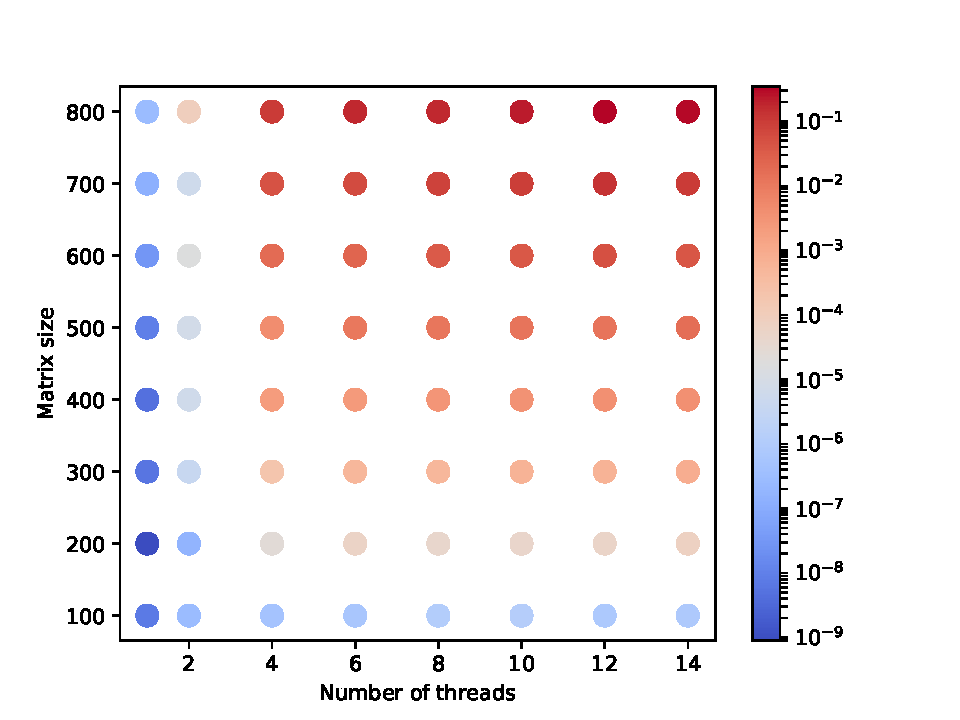
\includegraphics[width=100mm]{images/var_chunk_sizes.pdf}
	\caption{Variance of execution times as a function of features on Matrix Multiplication algorithm}
\end{figure}

 It would seem, according to this result, that when you add more threads and more iterations, the more variations you observe when measuring execution time for different chunk-sizes. However there is a problem with this result, the execution times are not all on the same scale. In fact the more iterations you have, the bigger the execution time. In that case, the execution time ranges from 0.005 to 2 seconds depending on the experiment. To solve this problem, the relative variance must once again be used. 

Here is a plot of the relative variance for all the same experiments:

\begin{figure}[H]
	\centering
	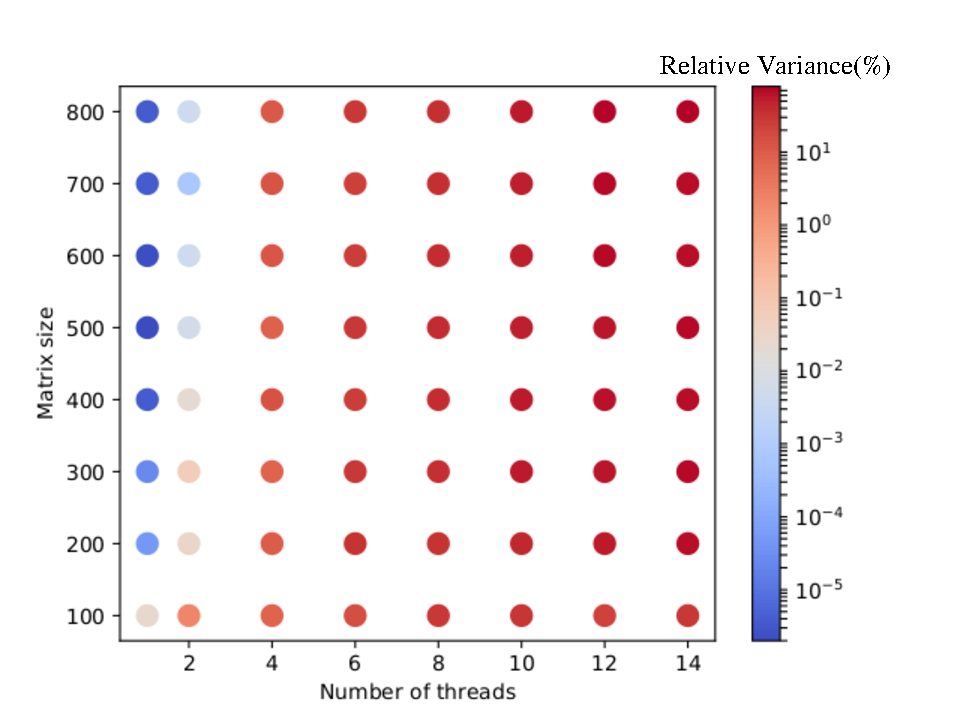
\includegraphics[width=100mm]{images/rel_var_chunk_sizes.pdf}
	\caption{Relative Variance (\%) of execution times as a function of features on Matrix Multiplication algorithm}
\end{figure}

As we can see, the relative variance depends highly on the number of threads. It appears that the lowest variance is obtained when using only one threads which makes sense since 1 thread is equivalent to sequential execution. Therefore, it has been decided that the number of threads would never be put to 1 because of the low relative variance between execution times. We can also see that by adding more threads, we add more variances in the execution times because an efficient use of these threads results in a significantly smaller execution time.

\subsubsection{Function analysis}
In this section, the focus will be on analyzing the function that will be approximated by machine learning

$$f:\{X_i\} \rightarrow cs_i$$

The data used to visualize this function is comprised 64 experiments of matrix multiplication with 100,200,300,400, 500,600,700,800 iterations and 1,2,4,6,8,10,12,14 threads. The chunk sizes candidates were $CS=\{0.005; 0.01 ;0.05; 0.1; 0.2; 0.5\}$

First of all, it is important to note that since when generating data with only a matrix multiplication function, the features <Number of Operations> <Number of Float Operations> and <Number of Comparison Operations> are a polynomial function of <Number of Iterations>

This means that of all 6 features, only 2 can be used (Deepest loop level is not necessary because it is the same for each matrix multiplication experiment). Here is a punctual color-map of the function with the current data.

\begin{figure}[H]
	\centering
	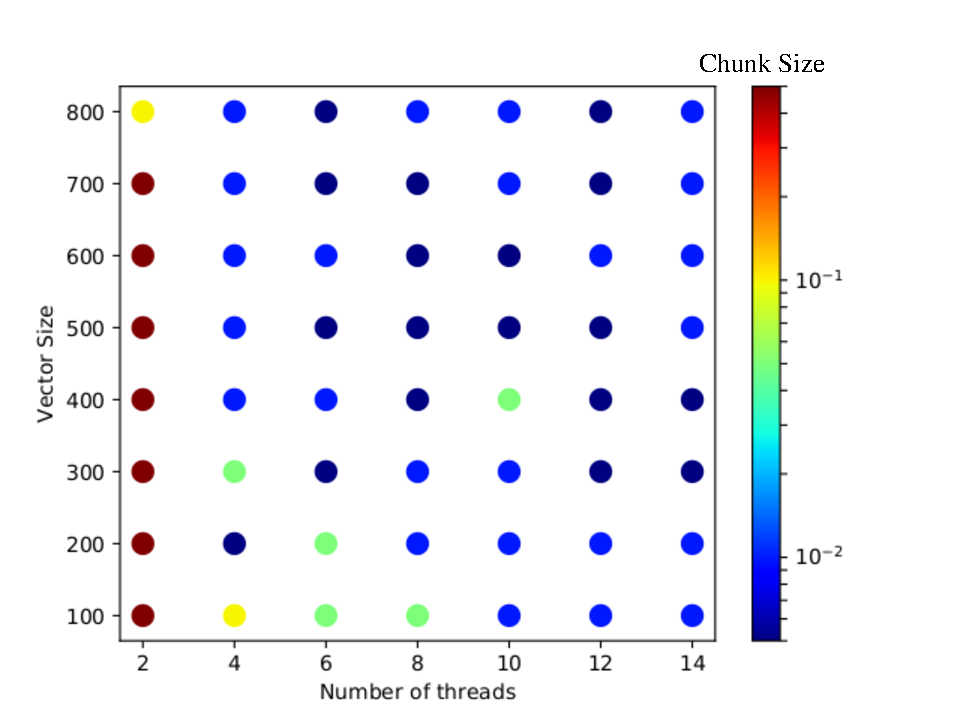
\includegraphics[width=120mm]{images/chunk_size_function_matrix.pdf}
	\caption{Optimal chunk size as a function of features on Matrix Multiplication algorithm}
\end{figure}

Number of threads has an impact on optimal chunk size For 100 iterations where we can see a steady decrease of chunk size with respect to number of treads. However for bigger matrices, the function oscillates. These oscillations are caused by the fact that execution times between 0.005 and 0.01 are very close. Here is a table of some execution times to show my point. (Note 0.2 was remove because it was never selected)

\begin{table}[h]
	\centering
	\caption{Execution times for 5 experiments of Matrix multiplication}
	\label{my-label}
	\begin{tabular}{|c|c|c|c|c|}
		\hline
		0.005& 0.01           & 0.05 & 0.1 & 0.5 \\ \hline
		0.221386 & 0.219532  & 0.247906    & 0.253246        & 0.629754 \\ \hline
		0.229569 & 0.229047 & 0.238892   & 0.422549        & 1.02871  \\ \hline
		0.168765 & 0.166738  & 0.2141   & 0.4157       & 1.0294  \\ \hline
		0.122448 & 0.121981  & 0.136015    & 0.260424        & 0.709034 \\ \hline
		0.0179531 & 0.0177467 & 0.0181951  & 0.0337951        & 0.082139 \\ \hline
	\end{tabular}
\end{table}

Here we can see than in all experiments, the execution times for 0.01 and 0.005 are very close. In fact the relative difference is around $1\%$ in average. The oscillations are caused by the fact that the time difference between 0.005 and 0.01 is smaller than the noise.

Here are some way we try to remove the oscillations

1-Matrices size is too small and therefore execution times for certain chunk sizes are too close to be reliably distinguishable.

2-There is a missing dynamic feature that is causing the variations which seem uncorrelated to the 2 current features.

3- Some chunk size candidates are too close to be reliably distinguished so the choice of candidates could be optimized.
\
\subsubsection{First approach}

The first approach was to use bigger matrices of sizes:
100,200,400,600,800,1000,1500,
2000,2500 with chunk-size candidates $CS=\{0.0005;0.001; 0.005; 0.01; 0.05; 0.1;0.5\}$

\begin{figure}[H]
	\centering
	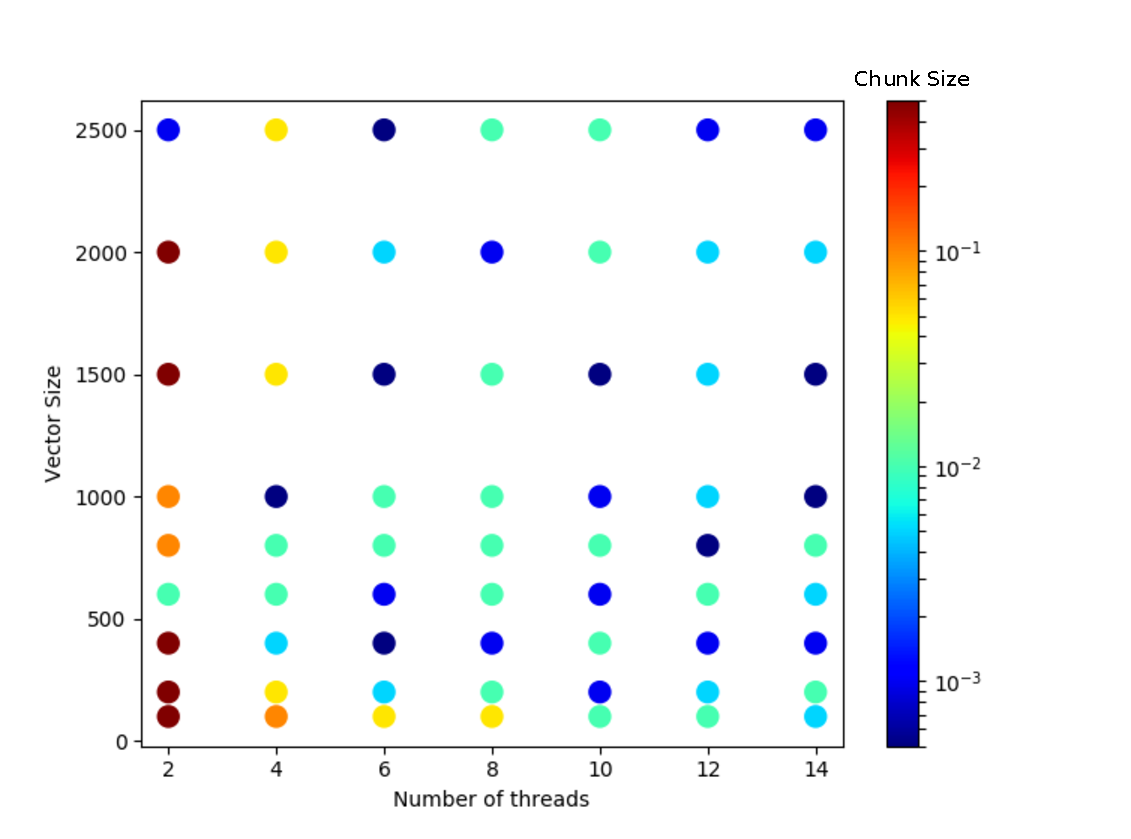
\includegraphics[width=120mm]{images/chunk_size_function_matrix_big.pdf}
	\caption{Optimal Chunk Size as a function of features on Matrix Multiplication algorithm with bigger matrices}
\end{figure}

We still observe oscillations so I decided to examine the execution times once more.

\begin{table}[h]
	\centering
	\caption{Execution times for 1000x1000, 1500x1500, 2000x2000 and 2500x2500 Matrices}
	\label{my-label}
	\begin{tabular}{|c|c|c|c|c|c|c|}
		\hline
		0.0005  & 0.001   & 0.005   & 0.01    & 0.05    & 0.1     & 0.5     \\ \hline
		NaN     & 1.06075 & 1.10638 & 1.01317 & 1.13454 & 1.15139 & 3.35216 \\ \hline
		NaN     & 3.33313 & 3.34309 & 3.33242 & 3.88524 & 3.93604 & 9.56364 \\ \hline
		7.91752 & 7.84541 & 7.8376  & 7.88513 & 9.22963 & 9.44594 & 22.4268 \\ \hline
		15.4564 & 15.5674 & 15.4928 & 15.4807 & 18.0824 & 18.2549 & 43.5778 \\ \hline
	\end{tabular}
\end{table}

It appears like once again, the execution times for the smaller chunk-sizes are very close, which explains the oscillations in the function. Having bigger matrices didn't seem to solve the issue.

\subsubsection{Second approach}

The idea would be to add the idle rate of the CPU's as a dynamic feature in the hope of having a better function.
This hasn't been done yet.

\subsubsection{Third approach}
By looking at table 2 and 3, it seems that chunk sizes which are different by a factor of two give very similar execution times while chunk sizes with a factor of 5 or more gave bigger differences. Here I will try to have a set of chunk size candidates where all consecutive chunk sizes are separated by the same multiplicative factor. First let's try with a factor 4. $CS=\{0.5;0.125;0.03125;0.0078125;0.001953125\}$. This means that the job will be split into 2,8,32,128,512 chunks.

Here is for small matrices

\begin{figure}[H]
	\centering
	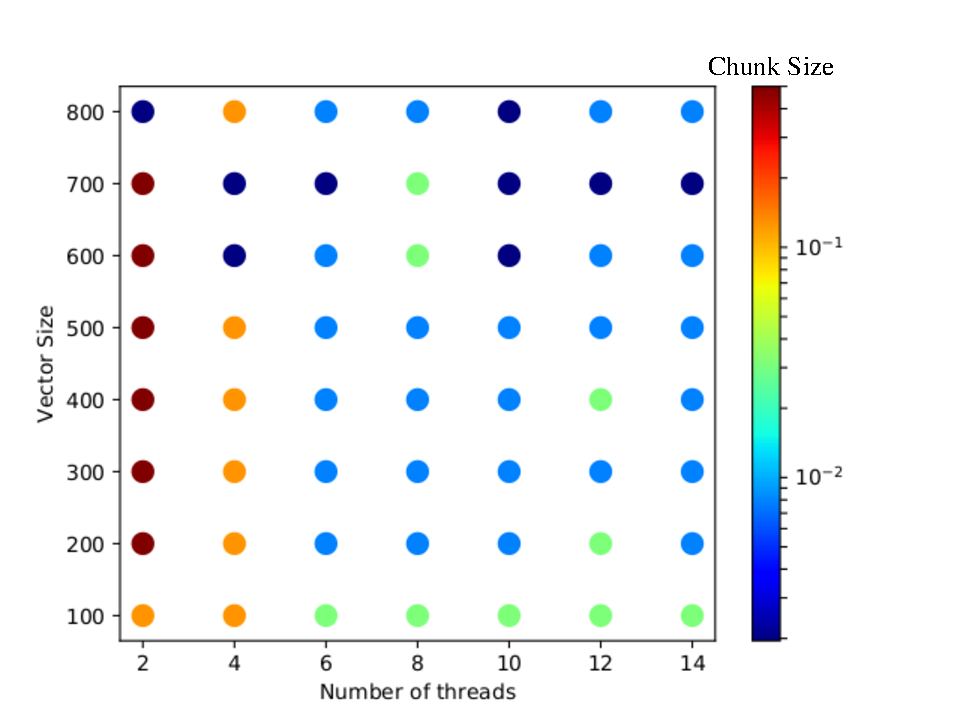
\includegraphics[width=120mm]{images/chunk_size_function_matrix_uniform_log.pdf}
	\caption{Optimal Chunk Size as a function of features with a set $CS$ uniform on logscale}
\end{figure}

And for bigger matrices
\begin{figure}[H]
	\centering
	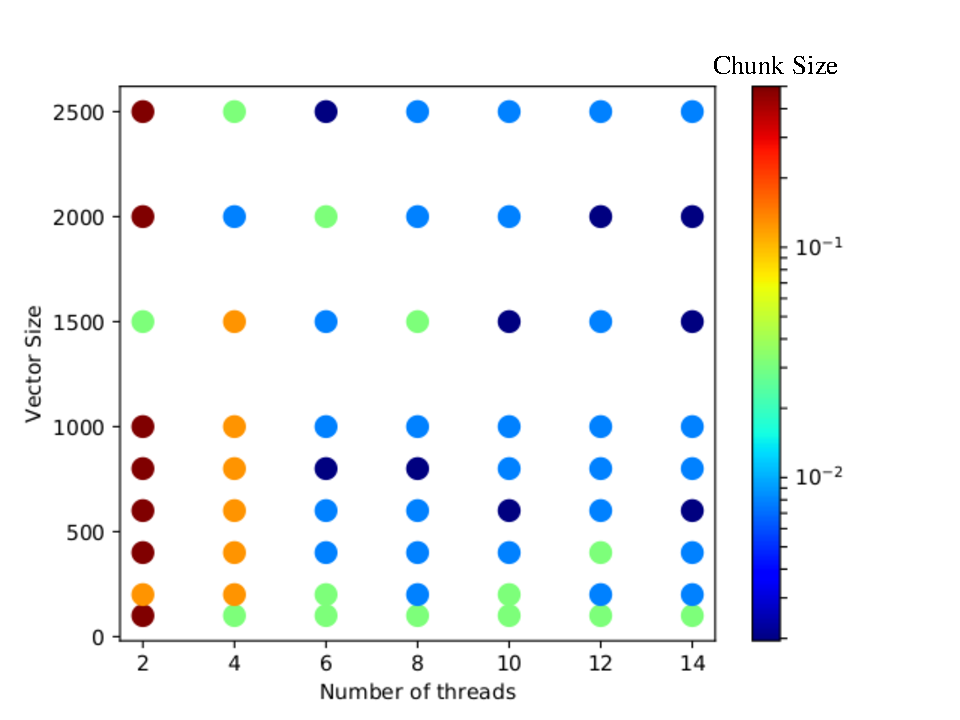
\includegraphics[width=120mm]{images/chunk_size_function_matrix_uniform_log_big.pdf}
	\caption{Optimal Chunk Size as a function of features on bigger matrices with a set $CS$ uniform on logscale }
\end{figure}

that result is very encouraging, We can see some reduction of the oscillations. The choice of candidates is still not optimal but we can see that choosing candidates is really important. Here is the results with 50 repetitions

\begin{figure}[H]
	\centering
	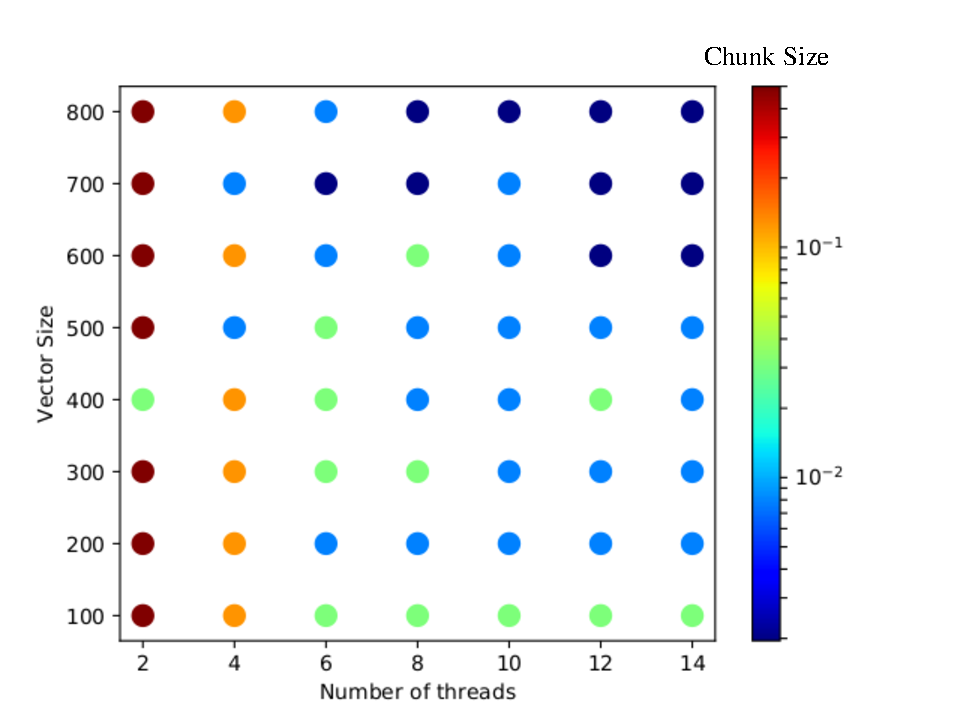
\includegraphics[width=120mm]{images/chunk_size_function_matrix_uniform_log_50rep.pdf}
	\caption{Optimal Chunk Size as a function of features with a set $CS$ uniform on logscale and 50 repetitions}
\end{figure}

This result is closer to what you would expect, the more threads and the bigger the Matrix, the more advantageous it becomes to split your job in many chunks. There is still some noise but it is unavoidable at this point. At least we can reduce it by changing the set of candidates.
\subsection{1D Stencil algorithm}

Another algorithm that was studied individually was 1D Stencil algorithm. It was studied because of its simplicity which make it different from Matrix Multiplication. Here the features <input size> can be renamed <vector size> since the 1D stencil is applied on a vector.
\newpage
\subsubsection{Function Analysis}

\begin{figure*}[h]
	\centering
	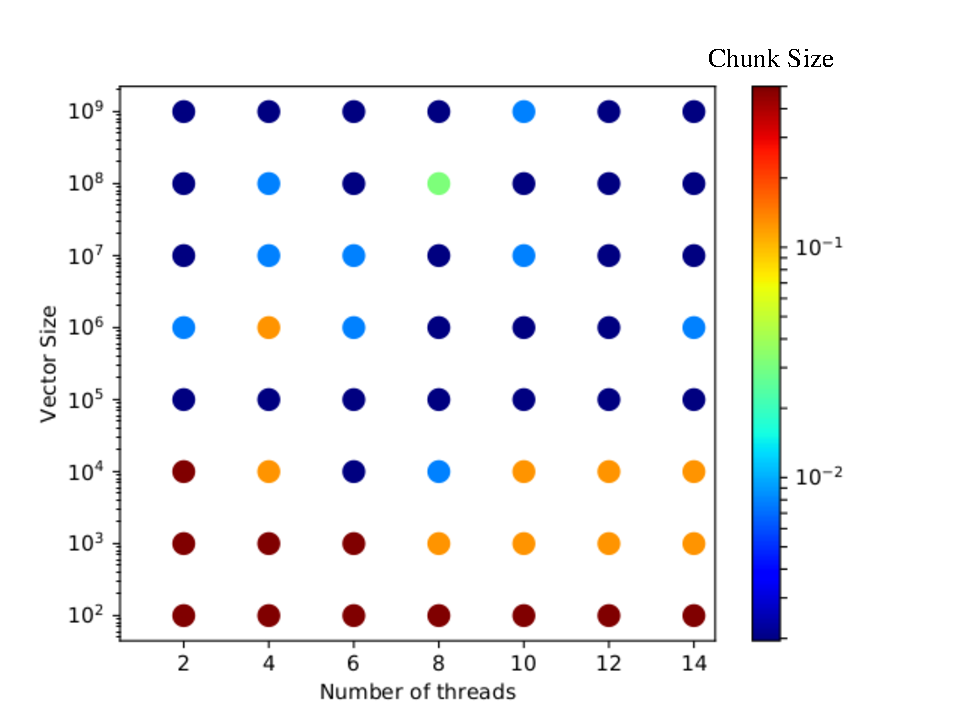
\includegraphics[scale=0.8]{images/stencil_function.pdf}
	\caption{Optimal Chunk Size as a function of features on Stencil algorithm with $CS$ uniform in logscale}
\end{figure*}
That result is very interesting because we really see a different behavior than with matrix Multiplication. Here the number of threads doesn't seem to have the same impact as Vector size which is the opposite of what was observed previously.

\newpage
\subsection{Data Set with many functions}
In this section, the focus will be on a bigger data set which is comprised of 278 experiments with many lambda functions. Here is a descriptions of all the functions used:



\begin{table}[h]
	\begin{tabular}{|c|c|c|}
		\hline
		\textbf{Name} & \textbf{Description} & \textbf{Numbers of iterations} \\ \hline
		Nothing() & Does Nothing & 10\textasciicircum{}7 \\ \hline
		Swap() & Swap elements between two vectors & \begin{tabular}[c]{@{}c@{}}100,1000,10000\\ 100000,100000\end{tabular} \\ \hline
		Stream() & Basic stream algorithm & 1000,10000,100000 \\ \hline
		Matrix\_Vector\_Mult() & Matrix Vector multiplication & \begin{tabular}[c]{@{}c@{}}100,500,1000\\ 5000,10000,20000\end{tabular} \\ \hline
		Dyadic() & Applies a dyadic product on two vectors & 100,1000,10000 \\ \hline
		Cosine() & \begin{tabular}[c]{@{}c@{}}Applies a cosine function on \\ each element of a given\\  vector using Taylor series\end{tabular} & \begin{tabular}[c]{@{}c@{}}100,1000,10000\\ 100000\end{tabular} \\ \hline
		Matrix\_Matrix\_Mult() & Matrix Matrix multiplication & \begin{tabular}[c]{@{}c@{}}100,500,1000,\\ 1500,2000,2500\end{tabular} \\ \hline
		Max() & \begin{tabular}[c]{@{}c@{}}Find the max of each column of a \\ 3 dimensional array\end{tabular} & \begin{tabular}[c]{@{}c@{}}1000,5000,10000,\\ 50000,100000\end{tabular} \\ \hline
		Tensor\_Generator() & Generates a tensor of dimension 4 & 100,200 \\ \hline
	\end{tabular}
	\caption{All functions used to generate 278 experiments}
\end{table}

Due to the difficulty of analyzing functions of more than 2-3 dimensions, this function has not been analyzed yet. However at some point it should be analyzed as this data-set is closer to what will be used in practice.
